\section{What survives diffusion noise: attenuation by statistical order}
\label{sec:theory}

Write $\gamma$ for the standard Gaussian on $\Reals^{\nsites}$, $\Hen{k}$ for the
probabilists' Hermite polynomials and $H_\nu(\vx)=\prod_i\Hen{\nu_i}(x_i)$ for their
products, of degree $|\nu|$. The channel \cref{eq:channel} acts on Hermite moments
diagonally.

\begin{theorem}[Hermite attenuation]
\label{thm:hermite}
For every multi-index $\nu$ with $\E_{\Pz}|\va|^{|\nu|}<\infty$,
$\;\E_{\Pt}[H_\nu(\vx_t)]=e^{-|\nu|t}\,\E_{\Pz}[H_\nu(\va)]$.
\end{theorem}
\begin{proof}
Mehler's identity $\E_{z}[\Hen{n}(\alpha a+\sqrt{1-\alpha^2}\,z)]=\alpha^n\Hen{n}(a)$ for
$z\sim\normal{0}{1}$ follows from the generating function
$e^{sx-s^2/2}=\sum_n\Hen{n}(x)s^n/n!$; coordinates are independent given $\va$, and
$\alpha=e^{-t}$.
\end{proof}
Nothing here requires $\Pz/\gamma\in L^2(\gamma)$---which fails for the Laplace chain and,
because $\lmax(\Sig_0)>2$, for the Gaussian chain at $\corr=0.85$---only finite moments.
Two consequences are exact at every $t$: cumulants of order $m\ge3$ scale as $e^{-mt}$
(Gaussian noise has none), and the degree-4 Hermite moments of two variance-matched laws
differ exactly by their fourth-cumulant tensors $\kfour$, attenuated by $e^{-4t}$.
Correlation lives at degree two and decays as $e^{-2t}$; non-Gaussian shape first appears
at degree four and decays as $e^{-4t}$. \emph{Diffusion noise is a low-pass filter on
statistical order.}

The consequence for scores and for learning is an expansion in the signal-to-noise
ratio $e^{-2t}$. Let $s=e^{-t}\vx/\Dt$, $b=e^{-2t}/\Dt$ and
$\Lambda(s,b)=\log\E_{\Pz}\exp(s\cdot\va-b|\va|^2/2)$, so that
$\log\Pt(\vx)=\log\gamma_{\Dt}(\vx)+\Lambda(s,b)$ and
$\score=-\vx/\Dt+(e^{-t}/\Dt)\nabla_s\Lambda$ exactly. Grading $\Lambda$ by order in
$e^{-t}$, its second-order part is the same for $\Pz$ and its covariance twin, and its
fourth-order part differs by a term linear in $\kfour$.

\begin{theorem}[Order-by-order information decay]
\label{thm:decay}
Let $\Pz$ have finite eighth moments and covariance $\Sig_0$, let $\Sgauss$ be the score
of its covariance twin, and let $\lmax=\lmax(\Sig_0)$. As $t\to\infty$,
\begin{align}
  \E_{\Pt}\lVert\score-\Sgauss\rVert^2
   &= \tfrac{1}{6}\Frob{\kfour}^2\,e^{-8t}\bigl(1+\epsilon_t\bigr),
  \label{eq:scoregap}\\
  I_t(\theta)&= \tfrac12\Frob{\partial_\theta\Sig_0}^2\,e^{-4t}\bigl(1+\epsilon_t\bigr)
  \ \ \text{if }\partial_\theta\Sig_0\neq0,
  \label{eq:info2}\\
  I_t(\theta)&= \tfrac1{24}\Frob{\partial_\theta\kfour}^2\,e^{-8t}\bigl(1+\epsilon_t\bigr)
  \ \ \text{if }\partial_\theta\Sig_0=0,\ \partial_\theta\kfour\neq0,
  \label{eq:info4}
\end{align}
with $\epsilon_t=O(e^{-2t}\lmax)$,
where $I_t(\theta)=\E_{\Pt}[(\partial_\theta\log\Pt)^2]$ is the Fisher information one
noised sequence carries about a parameter $\theta$ of $\Pz$, and $\Frob{\cdot}$ is the
Frobenius norm of the matrix or symmetric 4-tensor. For a Gaussian chain
\cref{eq:info2} is exact at every $t$ with
$I_t=\tfrac12\operatorname{tr}(\Sig_t^{-1}\partial_\theta\Sig_t\Sig_t^{-1}\partial_\theta\Sig_t)$.
\end{theorem}
The information statements \cref{eq:info2,eq:info4} are the diffusion-time form of a
principle established for low-SNR latent-variable models: the log-likelihood expands in
powers of the SNR with the order-$k$ term carrying $k$-th-moment information
\citep{katsevich2023likelihood,perry2019sample,bandeira2023estimation}, and Fisher
information about directions first identifiable at moment order $k$ scales as
$\mathrm{SNR}^k$ \citep{balanov2026gmm}; with $\mathrm{SNR}_t\simeq e^{-2t}$ these are
\cref{eq:info2,eq:info4}. The cumulant attenuation behind \cref{thm:hermite} is also
written down for the forward process by \citet{aarts2025cumulants}. What is new is
the score-level statement \cref{eq:scoregap} with its constant, made interpretable by
\cref{prop:lmmse}; the crossover below; and the exact verification and learning
consequences that follow. The proof (\cref{app:proofs}) expands $\Lambda$ to fourth order, takes the
$\gamma$-second moment of the leading Hermite term by Wick's theorem, and bounds the
remainder by the moment condition; the scalar leading term of \cref{eq:scoregap} is
$(\kfour/6)\Hen{3}(x)e^{-4t}$. The leading orders of a degree-2 and a degree-4 coordinate
do not couple, because $\Hen{2}$ and $\Hen{4}$ are $\gamma$-orthogonal, so the
\emph{efficient} information of a shape coordinate after the nuisance coordinates are
estimated has the same rate as its raw information.

\begin{remark}[General order]
The same grading gives, for a coordinate whose lowest non-vanishing Hermite footprint has
degree $m$, $I_t(\theta)\propto e^{-2mt}$: the leading term of $\partial_\theta\log\Pt$ is
$e^{-mt}$ times a degree-$m$ Hermite polynomial, whose $\gamma$-second moment is a
constant. The constants are explicit for $m=2,4$ above.
\end{remark}

\begin{corollary}[Sample complexity by order]
\label{cor:samples}
Estimating a covariance coordinate to fixed precision from sequences observed at level
$t$ needs $\nseq\propto e^{4t}$ of them; a shape coordinate needs $\nseq\propto e^{8t}$.
The ratio of the two informations is $\propto e^{-4t}$.
\end{corollary}

\paragraph{Where the asymptote begins.}
The expansion parameter is $e^{-2t}\lmax(\Sig_0)$, not $e^{-2t}$, with
$\lmax\le(1+\corr)/(1-\corr)$ for the chain. Below
$\tstar=\tfrac12\log\lmax(\Sig_0)$ the long-wavelength covariance modes are still of
order one and the rates are shallower; above it the exponents of \cref{thm:decay} hold.
At $\corr=0.85$, $\tstar=\gaussTstareightfive$: a strongly correlated chain keeps its
correlation information longer, and any measurement stopped near $\tstar$ sees slopes
short of $-4$ and $-8$.

\begin{figure*}[t]
  \centering
  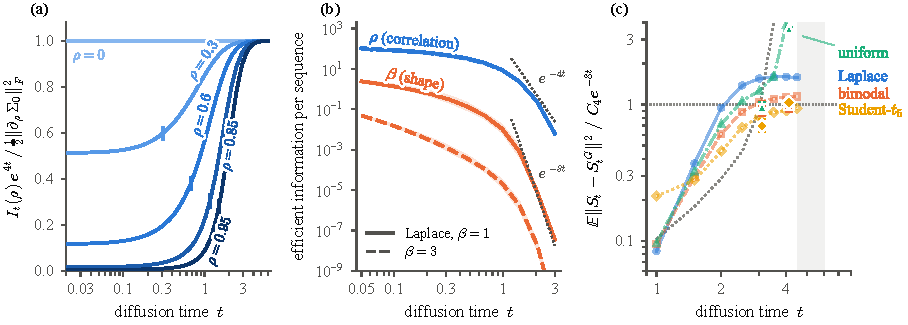
\includegraphics[width=\textwidth]{fig_theory.pdf}
  \caption{\textbf{What survives diffusion noise.}
  (a)~Exact Fisher information of the Gaussian chain about $\corr$, scaled by its
  predicted asymptote $\tfrac12\Frob{\partial_\corr\Sig_0}^2e^{-4t}$, for five $\corr$;
  every curve reaches~1, and the tick on each marks $\tstar(\corr)$.
  (b)~Efficient information per noised sequence about the correlation coordinate $\corr$
  (degree~2) and the shape coordinate $\beta$ (degree~4) of the generalised-Gaussian
  chain, from tree-exact inference and Fisher's identity, $\shapeChains$ sequences
  $\times\,\shapeReps$ replicates (bands: replicate range); guides $e^{-4t}$ and $e^{-8t}$.
  Above $\tstar$ the fitted slopes are $\shapeSlopeRhoone$ ($\corr$) and
  $\shapeSlopeBetathree$ ($\beta$, at $\beta=3$).
  (c)~The price of second-order closure: $\E\lVert\score-\Sgauss\rVert^2$ measured by
  tree-exact BP, divided by the predicted $\tfrac16\Frob{\kfour}^2e^{-8t}$, for four
  innovation families. Laplace and the bimodal mixture reach the constant to within
  $\closureRatiolaplacetthreepzero$--$\closureRatiobimodaltfourpzero$; Student-$t_5$, whose sixth
  moment is infinite, departs as the moment condition predicts; the uniform family reaches
  the floor of double precision near $t=3.5$.}
  \label{fig:theory}
\end{figure*}

\paragraph{Verification with the exact score.}
\Cref{fig:theory} tests \cref{thm:decay} where nothing has to be approximated. For the
Gaussian chain the closed form gives slope $\gaussSlopeRhoeightfive$ above $\tstar$ at
$\corr=0.85$ and the scaled information $\gaussScaledRhoeightfivetone$, $\gaussScaledRhoeightfivettwo$,
$\gaussScaledRhoeightfivetthree$ at $t=1,2,3$. For the non-Gaussian chain the shape information,
estimated from per-sequence scores obtained by Fisher's identity through the tree-exact
recursion, falls with slope $\shapeSlopeBetatwo$ ($\beta=2$) and $\shapeSlopeBetathree$
($\beta=3$) above $\tstar$, against the predicted $-8$, while the correlation
information falls with slope $\shapeSlopeRhotwo$ against $-4$; the kinked Laplace density
($\beta=1$) reaches the quadrature floor of the outer-product estimate near $t=2.5$.
The closure gap on the Laplace chain decays with slope $\closureSlopeSqlaplace$ and
reproduces the constant $\tfrac16\Frob{\kfour}^2$ ($\closureCfourlaplace$ for
$\nsites=32$) to $\closureRatiolaplacetthreepzero$ at $t=3$. The theorem also explains a
measurement the previous literature on this model reported as a discrepancy: information
slopes of about $-3$ and $-6$ obtained over $t\le1.6$ are the pre-asymptotic values below
$\tstar=\gaussTstareightfive$, not a failure of the $e^{-4t}$, $e^{-8t}$ law.

\paragraph{What this says about score learning.}
An estimator that carries only second-order structure cannot go below the LMMSE floor
$\lVert\score-\Sgauss\rVert$, which on the Laplace chain at $\corr=0.85$ is
$\lmmseFloorLaplace$ of the score energy pooled over the twelve-level schedule and
$\lmmseLowestLaplace$ at the lowest level (\cref{app:oracles}). A learner that recovers the
fourth-order structure has, by \cref{cor:samples}, $e^{4t}$ fewer effective samples per
sequence at level $t$ than one that recovers only covariance: the twelve-level schedule
is, for shape, effectively a four-level one. Both facts organise the experiments of
\cref{sec:experiments}.
